\section{Introduction}

The black Sigatoka disease caused by the fungus \emph{Mycosphaerella
  fijiensis Morelet} is the major pathological problem of banana and
plantain crops in Central America, Panama, Colombia and Ecuador, as well as in
many parts of Africa and Asia \citep{MarinVargas1995}.

This disease attacks the plant leaves producing a rapid deterioration
of the leaf area. It affects the growth and productivity of the plants
due to the impairment of the photosynthetic process.  Furthermore, it
causes a reduction in the quality of the fruit, and promotes premature
ripening of bunches, which is the major cause of product losses
associated with the black Sigatoka.

For these reasons, warning systems have been developed to detect the
disease and monitor its progress.  For instance, the early warning
system developed by \citet{ganry1983} and modified by
\citet{ganry1972} for the control of the yellow Sigatoka in Cameroon,
was later adapted by \citet{Ternesien1985} and \citet{foure1988} for
the black Sigatoka.

This biological warning system is based on weekly observations of the
disease progression on young leaves of the plant.
%
\figref{fig:diseasestages} shows an example of three progressive
stages of the black Sigatoka.
%	 
\begin{figure}[ht] 
\centering
\begin{tabular}{c@{\;}c@{\;}c}
  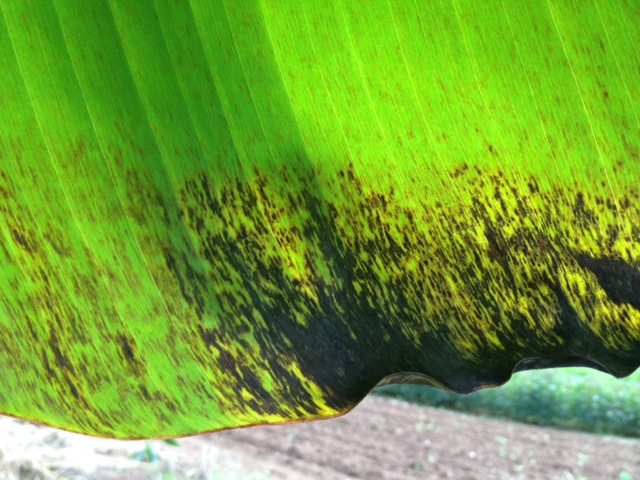
\includegraphics[width=.32\linewidth]{Roya_a} &
  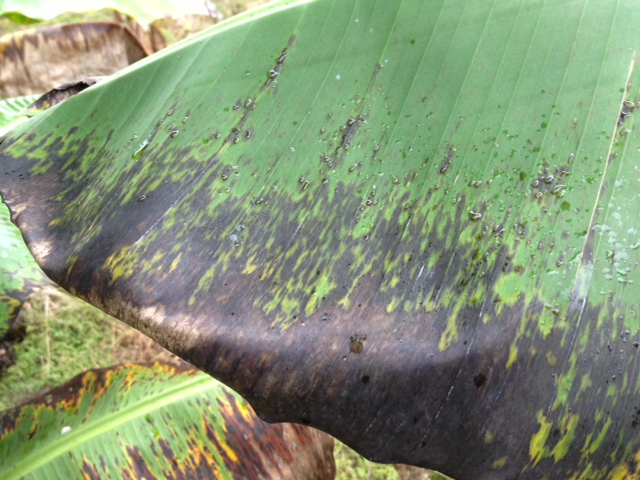
\includegraphics[width=.32\linewidth]{Roya_b} &
  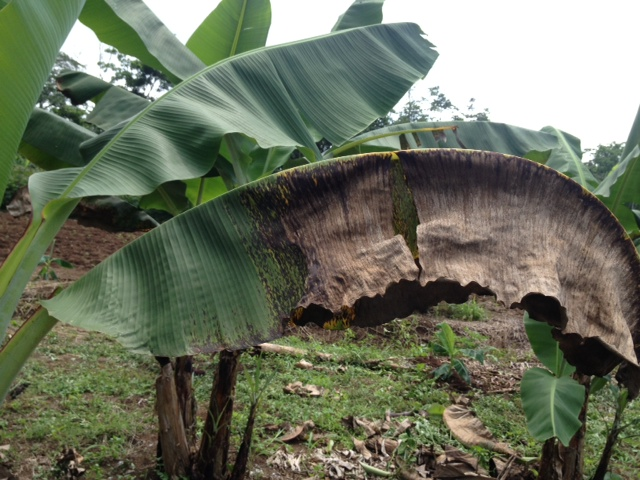
\includegraphics[width=.32\linewidth]{Roya_c} \\
  (a) & (b) & (c) 
\end{tabular}
\caption{Examples of three disease stages of the black Sigatoka. 
(a)~Initial stage. (b)~Intermediate stage, and (c)~Advanced stage.} 
\label{fig:diseasestages} 
\end{figure}

The disease progression is then quantified according to Fouré's scale
of the symptom stages \citep{foure1988} by means of numeric
coefficients that describe the degree of incidence and the severity of
the disease development.  These coefficients are then used to
calculate two variables: gross sum and state of evolution.

The gross sum is based on the present disease progression stage and
the numeric coefficients, which increase with the progression of
the symptoms and the juvenility of the leaf.
%
The state of evolution is calculated using the gross sum and the
foliar emission period.
%
Decades ago threshold levels on these variables were used as a guide
to plan the spray schedules.  Nowadays the fluctuation of these two
variables seems to better suggest appropriate times to spray
\citep{Marinetal2003}.

In Costa Rica the black Sigatoka is frequently treated with
chemical fungicides.
%
Depending on the zone of production and the weather conditions,
45--55~cycles/year of fungicide applications are required to keep this
disease under control and to produce the expected fruit quality for the
international markets.
%
This represents a cost per hectare per year in the range from US\$1600
to US\$2000; about 0.64--0.80 cents of the production costs for a
18.14\,kg box, which overall corresponds to 10\%--12\% of the total
production costs.

The past and present rates of disease development can in principle be
used to predict its future behavior and to determine if a particular
fungicide spray program will be able to effectively treat the disease
in an economically affordable way \citep{ChuangJeger1987}.
%
Phytopathological studies point out that climate has a major effect on
the development of the black Sigatoka, where the main variables
affecting it are precipitation, temperature, relative humidity and
wind \citep{MarinVargas1995}.  It can be expected that patterns in
these variables correlate with the disease development and hence its
automated discovery can support decision-making in the control of crop
diseases.

In this work, we compare four machine learning techniques to predict
the development rate of the black Sigatoka disease: support vector
regression (SVR), echo state networks (ESN), elastic net regression 
and ordinary least squares linear regression,
using input variables: maximal air temperature, minimal air temperature,
 mean air temperature, mean relative humidity, minimal relative humidity, 
 maximal relative humidity, mean solar radiation, sum of precipitation, 
 maximal wind speed and mean speed wind, to predict the evolution stage 
 in the biological warning system. 

 The main findings were: 1) The highest R2 was 60\% 2) The highest R2 
 were reached with linear models like support vector regression with 
 linear kernel, 3) As little as three meteorological variables can 
 be used because of the correlations detected among variables. 

The outline of the paper is as follows: Section~\ref{sec:related}
presents related works and Section~\ref{sec:techs} summarizes the
machine learning techniques selected for the analysis. In
Section~\ref{sec:data} we present the methodology used in this study
and describe data used for its verification.  The results and their
discussion are presented in section~\ref{sec:results}.  The
Section~\ref{sec:concl} concludes this article and presents lines for
future works.
%
